\newpage
\section{Analisi complessiva}

\subsection{Struttura}
Come si può evincere dal resto dell'analisi, la struttura del sito è piuttosto confusionaria, in primis la homepage. Lo stile non è unico e uniforme, e questo può far spazientire l'utente ma, soprattutto, rischia di confondere le idee e compromettere lo schema mentale che l'utente si fa alla prima vista della pagina. \\
La visualizzazione delle news in homepage, per quanto utile e, in parte, funzionale, non possiede una struttura lineare, e può perciò essere di difficile interpretazione a un occhio distratto. L'alternarsi di immagini piccole e grandi e di anteprime "a griglia" e a lista trasmette inoltre una sensazione di poca cura dei particolari e poca attenzione alla leggibilità del sito. \\
Un simile discorso si può fare per quanto riguarda le pagine interne: la scelta fatta è stata quella di privilegiare le immagini, ponendo una grande immagine di copertina all'inizio di ogni articolo; questo inficia sui timer degli utenti, i quali dedicheranno poi meno tempo a leggere il contenuto, a causa del tempo sprecato nello scroll della pagina.

\subsection{Pubblicità}
Il sito possiede due slot per l'inserimento di pubblicità, per il momento ancora vuoti (pubblicizzano infatti lo slot stesso).

\vspace{30pt}
\begin{figure}[htbp]
\begin{center}

\includegraphics[width=35em]{img/pubblicita1}
\caption{Pubblicità in alto}
\end{center}
\end{figure}
\vspace{30pt}

\begin{figure}[htbp]
\begin{center}

\includegraphics[width=10em]{img/pubblicita2}
\caption{Pubblicità a lato dell'articolo}
\end{center}
\end{figure}
\vspace{30pt}

Le posizioni sono rispettivamente in alto in centro (affianco al logo) e sul lato destro degli articoli. Si può dire poco a proposito poiché vuoti, ma le posizioni sono comunque ottimali: %GUARDARE SUL QUADERNO I POSIZIONAMENTI

\subsection{404}
Il sito prevede una \textit{pagina di 404}, molto utile a tranquillizzare l'utente in caso in cui manchi una risorsa cercata.

\vspace{30pt}
\begin{figure}[htbp]
\begin{center}
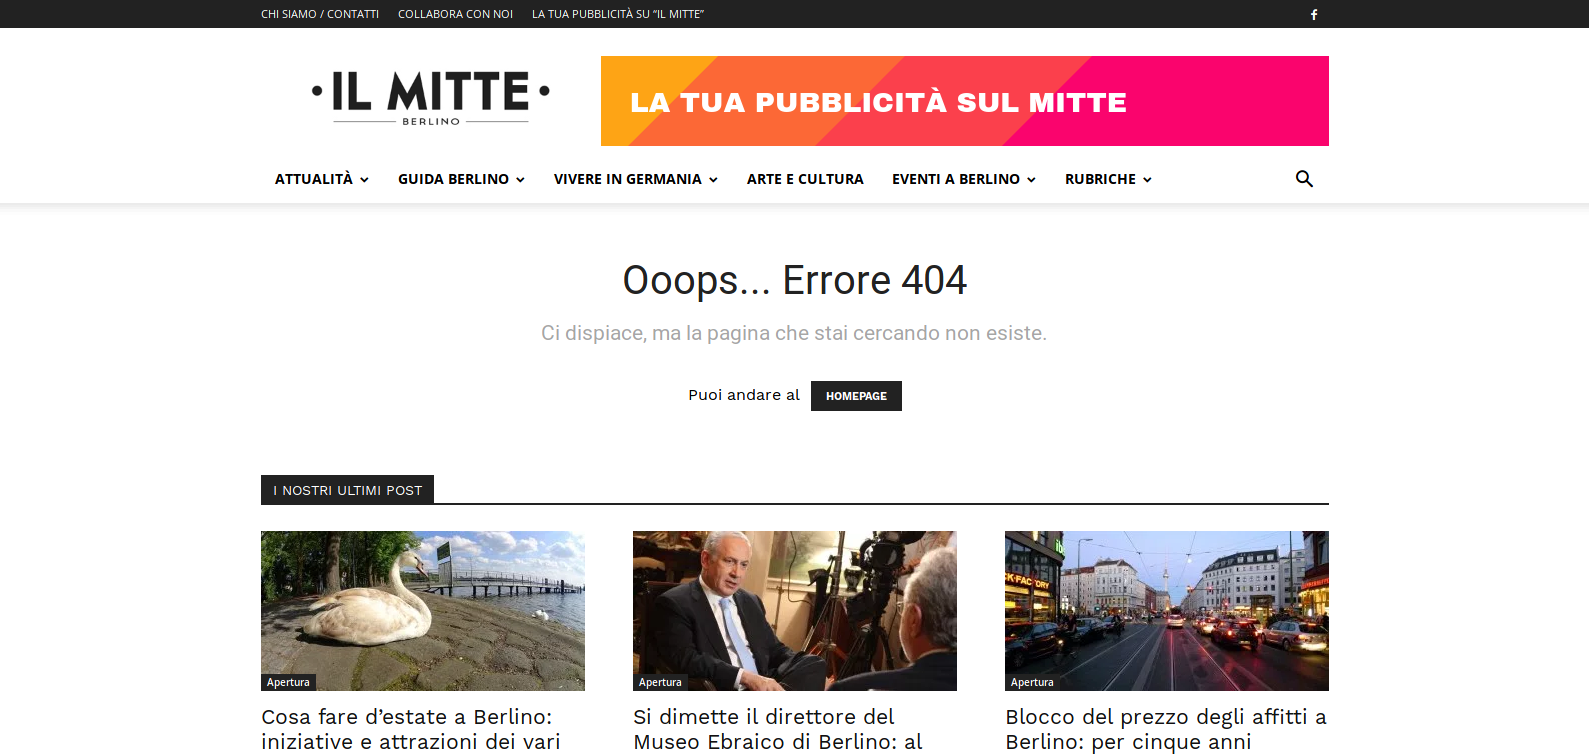
\includegraphics[width=30em]{img/404}
\caption{La pagina d'errore}
\end{center}
\end{figure}
\vspace{30pt}

La pagina non è particolarmente curata, ma svolge il suo lavoro; propone infatti all'utente più scappatoie dalla pagina, poiché si può tornare alla Homepage oppure saltare direttamente a uno degli ultimi sei articoli pubblicati.